
 \documentclass[twocolumn,letterpaper]{igs} 

\usepackage{lmodern}
\usepackage{amsmath,amssymb,amsthm}
\usepackage{graphicx}
\usepackage{natbib} 
\usepackage{wrapfig}
\usepackage{enumitem}
\usepackage{multirow}
\usepackage{tabularx}
\usepackage{booktabs}


\begin{document}

%%%%%%%%%%%%%%%%%%%%%%%%%%%%%%%%%
%	METHODS
%%%%%%%%%%%%%%%%%%%%%%%%%%%%%%%%%


\section{Methods}

Estimating accumulation involves transforming snow depth and density measurements to distributed estimates of snow water equivalent (SWE). We use four main processing steps that obtain (1) measurements, (2) distributed density, (3) grid cell average and (4) interpolated SWE. To estimate the specific winter surface mass balance (WSMB) we calculate the mean SWE for a grid cell from the estimated distributed SWE. 

\subsection{Measurements}

\begin{figure*}
	\centering
	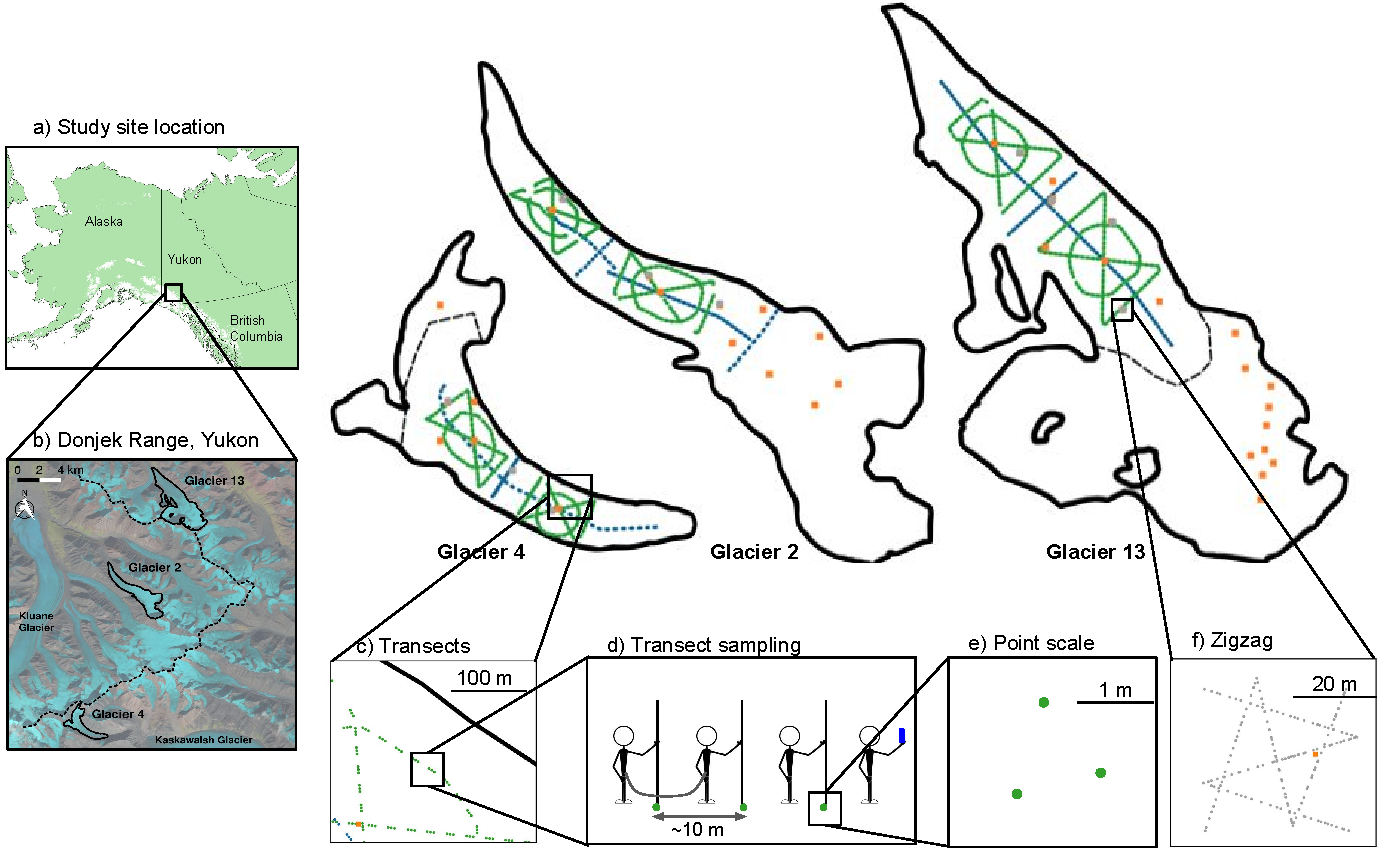
\includegraphics[width =\textwidth]{Sampling.pdf}\\
	\caption{Sampling design for Glaciers 4, 2 and 13, located in the the Donjek Range, Yukon (a,b). Centreline and transverse transects are shown in blue dots, hourglass and circle design are shown in green dots and zigzag measurements are shown as grey dots (c). Linear and curvilinear transects typically consist of sets of three measurement locations, spaced $\sim$10 m apart (d). At each measurement location, three snow depth observation are made (e). Orange squares are locations of snow density measurements. }
	\label{fig:Sampling}
\end{figure*}

The estimated SWE is the product of the snow depth and density. Snow depth is generally accepted to be more variable than density \citep{Elder1991, Clark2011, Lopez2013} so we chose a sampling design with relatively small measurement spacing along transects that resulted in a ratio of approximately 55:1 snow depth to snow density measurements. The sampling design attempted to capture depth variability at multiple spatial scales and to account for known variation with elevation. Our sampling design is created to avoid bias, be space filling within the ablation area and minimize distance travelled \citep{Shea2010}.

We measured accumulation at three glaciers along the precipitation gradient in the St. Elias Mountains, Yukon \citep{Taylor1969} in an attempt to account for range-scale variability \citep{Clark2011}. We measured accumulation on Glaciers 4, 2, and 13 (naming adopted from \cite{Crompton2016}), which are located increasingly far from the head of the Kaskawalsh Glacier (Figure \ref{fig:Sampling}b). Snow depth was measured along linear and curvilinear transects to encompass basin-scale variability. At each measurement location, three values of snow depth were recorded to account for point-scale variability \citep{Clark2011}.  We selected centreline and transverse transects with sample spacing of $10-60$ m (Figure \ref{fig:Sampling}d) to capture previously established correlations between elevation and accumulation \citep{Machguth2006, Walmsley2015} as well as accumulation differences between ice-marginal and center accumulation. We also implemented an hourglass and circle design (Figure \ref{fig:Sampling}), which allows for sampling in all directions and easy travel (Parr, C., 2016 personal communication). At each measurement location, we took $3-4$ depth measurements (Figure \ref{fig:Sampling}e), resulting in more than 9,000 snow depth measurements throughout the study area. 

Our sampling campaign involved four people and occurred between May 5 and 15, 2015, which corresponds to the historical peak accumulation in the Yukon (Yukon Snow Survey Bulletin and Water Supply Forecast, May 1, 2016). While roped-up for glacier travel, the lead person used a hand-held GPS (Garmin GPSMAP 64s) to navigate as close to the predefined transect measurement locations as possible (Figure \ref{fig:Sampling}). The remaining three people used 3.2 m aluminium avalanche probes to take $3-4$ snow depth measurements within $\sim$1 m of each other. Each observer was approximately 10 m behind the person ahead of them along the transect line. The location of each set of depth measurements, taken by the second, third and fourth observer, was approximated based on the recorded location of the first person. 

Snow depth sampling was primarily done in the ablation area to ensure that only snow from the current accumulation season was measured. Determining the boundary between snow and firn in the accumulation area, especially when using an avalanche probe, is difficult and often incorrect \citep{Grunewald2010,Sold2013}. We intended to use a firn corer to extract snow cores in the accumulation area but due to technical issues we were unable to obtain cohesive cores. The recorded accumulation area measurements were done either in a snow pit or with a Federal Sampler so that we could identify the snow-firn transition based on a change in snow crystal size and density. 

When estimating accumulation, snow depth variability at scales less than the grid-size of satellite derived elevation models is assumed to be caused by random effects that are unbiased and unpredictable \citep{Watson2006}. To capture grid-scale variability, we implemented a linear-random sampling design, termed `zigzag' \citep{Shea2010}. We measured depth at random intervals ($0.3 - 3.0$ m) along two `Z'-shaped transects within three to four $40\times40$ m squares (Figure \ref{fig:Sampling}c) aligned with randomly selected DEM grid cells distributed throughout the ablation zone.

Snow density was measured using a wedge cutter in three snowpits on each glacier. We collected a continuous density profile by inserting a $5\times5\times 10$ cm (250 cm$^3$) wedge-shaped cutter in 5 cm increments to extract snow samples and weighed the samples with a spring scale \citep[e.g.][]{Gray1981,Fierz2009}. Uncertainty in estimating density from snow pits stems from measurement errors and incorrect assignment of density to layers that could not be sampled (i.e. ice lenses and `hard' layers). 

While snow pits provide the most accurate measure of snow density, digging and sampling a snow pit is time and labour intensive. Therefore, a Federal Snow Sampler (FS) \citep{Clyde1932}, which measures bulk SWE, was used to augment the spatial extent of density measurements. A minimum of three measurements were taken at $7-19$ locations on each glacier and eight FS measurements were co-located with each snow pit profile. Measurements where the tube snow length was less than 90\% of the snow depth were assumed to be an incorrect sample and were excluded. Density values were then averaged for each location. 

During the field campaign there were two small accumulation events. The first, on May 6, also involved high winds so accumulation could not be determined. The second, on May 10, resulted in 0.01 m w.e accumulation at one location on Glacier 2. High temperatures and clear skies occurred between May 11 and 16, which we believed resulted in significant melt occurring on Glacier 13. The snow in the lower part of the ablation area was isothermal and showed clear signs of melt and snow metamorphosis. Total amount of accumulation and melt during the study period could not be estimated so no corrections were made. 

\subsection{Distributed density}

Measured density is interpolated to estimate SWE at each depth sampling location. We chose four separate methods that are commonly applied to interpolate density: (1) mean density over an entire range \citep[e.g.][]{Cullen2017}, (2) mean density for each glacier \citep[e.g.][]{Elder1991, McGrath2015}, (3) linear regression of density with elevation \citep[e.g.][]{Elder1998, Molotch2005} and (4) inverse-distance weighted density \citep[e.g.][]{Molotch2005}. 

When designing the sampling campaign we assumed that SP and FS densities could be combined so that we could have a more spatially distributed density data set. However, there is no correlation between co-located SP and FS densities (Figure \ref{fig:density_pitVStube}). Therefore, SP and FS measurements were used independently for each interpolation method, resulting in eight density interpolation options. 

\subsection{Grid cell average}

We average SWE values within each DEM-aligned grid cell. The locations of measurements have considerable uncertainty both from the error of the GPS unit ($2.7 - 4.6$ m) and the estimation of observer location based on the GPS unit. These errors could easily result in the incorrect assigning of a SWE measurement to a certain grid but this source of variability was not further investigated because we assume that SWE variability is captured in the zigzag measurements described below. There are no differences between observers (p$>$0.05), with the exception of the first transect on Glacier 4, so no corrections to the data based on observer are applied.

To encompass variability at spatial scales smaller than a DEM grid cell, we measured snow depth extensively ($135-191$ points) using a `zigzag' configuration (Figure \ref{fig:Sampling}c). Zigzag locations were randomly chosen within the upper ($\sim$2350 m a.s.l.), middle ($\sim$2250 m a.s.l.), and lower portions ($\sim$2150 m a.s.l.) of the ablation area of each glacier. We were able to measure a fourth zigzag on Glacier 13, which was located in the middle ablation area ($\sim$2200 m a.s.l.). SWE variability is assumed to be normally distributed about the mean SWE at a measured grid cell with a standard deviation equal to the average standard deviation of all zigzags on a glacier.

\subsection{Interpolated SWE}

SWE data were interpolated for each glacier using linear regression (LR), simple kriging (SK), as well as regression kriging (RK). Linear regressions relate observed SWE to grid cell values of DEM-derived topographic parameters \citep{Davis1986}. We chose to include elevation, distance from centreline, slope, aspect, curvature, ``northness'' and wind exposure/shelter in the LR. Topographic parameters were weighted by a set of fitted regression coefficients ($\beta_i$). Regression coefficients are calculated by minimizing the sum of squares of the vertical deviations of each data point from the regression line \citep{Davis1986}. The distributed estimate of SWE was found by using regression coefficients to estimate SWE at each grid cell. Specific WSMB was calculated as the mean SWE for each glacier ([m w.e.]). 

The goal of generating a LR is to predict SWE at unsampled grid cells and to tease out dominant relationships between accumulation and topographic parameters. Since snow depth data is highly variable, there is a possibility for the LR to fit to this data noise, a process known as overfitting. To prevent overfitting, cross-validation and model averaging were implemented. Cross-validation was used to obtain a set of $\beta_i$ values that have greater predictive ability. We selected 1000 random subsets (2/3 values) of the data to fit the LR and the remaining data (1/3 values) was used to calculate a root mean squared error (RMSE) \citep{Kohavi1995}. Regression coefficients resulting in the lowest RMSE were selected. Model averaging takes into account uncertainty when selecting predictors and also maximizes predictive ability \citep{Madigan1994}. Models were generated by calculating a set of $\beta_i$ for all possible combinations of predictors. Following a Bayesian framework, model averaging involves weighting all models by their posterior model probabilities \citep{Raftery1997}. To obtain the final regression coefficients, the $\beta_i$ values from each model were weighted according to the relative predictive success of the model, as assessed by the Bayesian Information Criterion (BIC) value \citep{Burnham2004}. BIC penalizes more complex models, which further reduces the risk of overfitting.

Topographic parameters are easy to calculate proxies for physical processes, such as orographic precipitation, solar radiation effects, wind redistribution and preferential deposition. We derived all parameters for our study from a SPOT-5 DEM ($40\times40$ m) \citep{Korona2009}. Elevation ($z$) values were taken from the SPOT-5 DEM directly. Distance from centreline ($d_C$) was calculated as the minimum distance between the Easting and Northing of the northwest corner of each grid cell and a manually defined centreline. Slope, aspect and curvature were calculated using the \texttt{r.slope.aspect} module in GRASS GIS software run through QGIS as described in \cite{Mitavsova1993} and \cite{Hofierka2009}. Slope ($m$) is defined as the angle between a plane tangential to the surface (gradient) and the horizontal \citep{Olaya2009}. Aspect ($\alpha$) is the dip direction of the slope and $\sin(\alpha)$, a linear quantity describing a slope as north/south facing, is used in the regression. Mean curvature ($\kappa$) is found by taking the average of profile and tangential curvature. Profile curvature is the curvature in the direction of the surface gradient and it describes the change is slope angle. Tangential curvature represents the curvature in the direction of the contour tangent. Curvature differentiates between mean-concave (positive values) terrain with relative accumulation and mean-convex (negative values) terrain with relative scouring \citep{Olaya2009}. ``Northness'' ($N$) is defined as the product of the cosine of aspect and sine of slope \citep{Molotch2005}. A value of -1 represents a vertical, south facing slope, a value of +1 represents a vertical, north facing slope, and a flat surface yields 0. The wind exposure/shelter parameter (Sx) is based on selecting a cell within a certain angle and distance from the cell of interest that has the greatest upward slope relative to the cell of interest \citep{Winstral2002}. Sx was calculated using an executable obtained from Adam Winstral that follows the procedure outlined in \cite{Winstral2002}. 

Our sampling design ensured that the ranges of topographic parameters covered by the measurements represented more than 70\% of the total area of each glacier (except for the elevation range on Glacier 2, which was 50\%). However, were were not able to sample at locations with extreme parameter values and the distribution of the sampled parameters generally differed from the full distribution.

Visual inspection of the curvature fields calculated using the DEM showed a noisy spatial
distribution that did not vary smoothly. To minimize the effect of noise on parameters sensitive to DEM grid cell size, we applied a $7\times7$ grid cells smoothing window to the DEM, which was then used to calculate curvature, slope, aspect and ``northness''.

Simple kriging (SK) estimates SWE values at unsampled locations by using the isotropic spatial correlation (covariance) of measured SWE to find a set of optimal weights \citep{Davis1986, Li2008}. SK assumes that if sampling points are distributed throughout a surface, the degree of spatial correlation of the observed surface can be determined and the surface can then be interpolated between sampling points. We used the DiceKriging R package \citep{Roustant2012} to calculate the maximum likelihood covariance matrix, as well as range distance and nugget. The range distance is a measure of data correlation length and the nugget is the residual that encompasses sampling-error variance as well as the spatial variance at distances less than the minimum sample spacing \citep{Li2008}. 

\subsection{Quantifying effects of variability}

We identify three major sources of variability within the process of translating snow measurements to WSMB. These variability sources encompass error and uncertainty within each processing step. When calculating distributed density, choice of density interpolation method is the largest source of variability. We therefore carry all density interpolation options forward in the estimation of WSMB. When calculating a grid cell average SWE, variability stems from a distribution of SWE values within each grid cell. We choose to encompass the SWE variability by generating a normal distribution of SWE values for each measured grid cell. The normal distribution has a mean equal to the grid cell average SWE and a standard deviation equal to the mean standard deviation of all zigzags on each glacier. When obtaining interpolated SWE, the best fit interpolation itself has variability based on the data that is used to fit the regression line or kriging surface. LR variability is represented by obtaining a multivariate normal distribution of possible $\beta_i$ values. The standard deviation of each distribution is calculated using the covariance of regression coefficients as outlined in \cite{Bagos2015}. SK variability is calculated using the DiceKriging package and is returned as an upper and lower 95\% confidence interval for SWE at each grid cell. We refer to the three variability sources as (1) density variability, (2) SWE variability and (3) interpolation variability. 

To quantify the effects of the three variability sources on the final WSMB estimate, we use a Monte Carlo experiment, which uses repeated random sampling to calculate a numerical solution \citep{Metropolis1949}. In our study, we randomly sample the distributions for SWE variability and interpolation variability and carry these values through the data processing steps to obtain a value of WSMB. First, the distribution of SWE values for each grid cell is independently sampled. Then, LR or SK is used to interpolate these SWE values. With the LR, a set of $\beta_i$ values and their distributions are calculated and the $\beta_i$ distributions are randomly sampled. These new $\beta_i$ values are used to calculate WSMB. With SK, a distribution of WSMB is calculated from the 95\% confidence interval kriging surfaces. Density variability is accounted for by repeating the process for each density interpolation method. This random sampling process is done 1000 times, which results in a distribution of possible WSMB values based on variability within the data processing.
 

%%%%%%%%%%%%%%%%%%%%%%%%%%%%%%%%%%%%%%%%%%%
%%  RESULTS 
%%%%%%%%%%%%%%%%%%%%%%%%%%%%%%%%%%%%%%%%%%%
\section{Results}

\subsection{ Measurements}

\begin{figure}
	\centering
	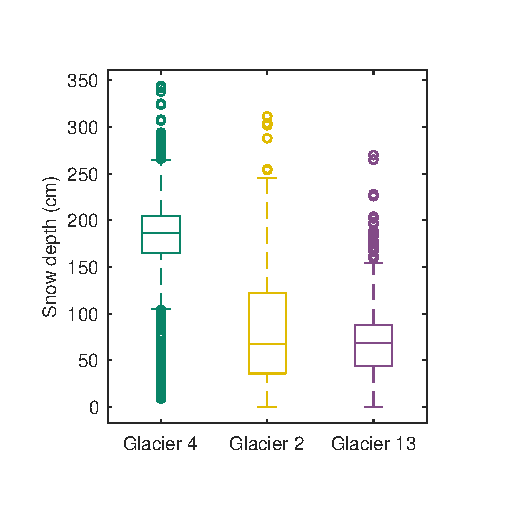
\includegraphics[width =0.5\textwidth]{DepthBoxplot.pdf}\\
	\caption{Boxplot of measured snow depth on Glaciers 4, 2 and 13. The box shows first quartiles, the line within the box indicates data median, bars indicate minimum and maximum values (excluding outliers), and circles show outliers, which are defined as being outside of the range of 1.5 times the quartiles (approximately $\pm2.7\sigma$). }
	\label{fig:DepthBoxplot}
\end{figure}

A wide range of snow depth is observed on all three study glaciers (Figure \ref{fig:DepthBoxplot}). Glacier 4 has the highest mean snow depth and a high proportion of outliers, indicating a more variable snow depth overall. Glacier 13 has the lowest mean snow depth and a narrower distribution of observed values. At each measurement location, the median range of measured depths ($3-4$ points) as a percent of the mean depth at that location is 2\%, 11\%, and 12\%, for Glaciers 4, 2 and 13, respectively. 

Mean SP and FS density values are within one standard deviation of each other for each glacier and over all three glaciers. The standard deviation of glacier-wide mean density is less than 10\% of the mean density. However, FS densities have a larger range of values ($227-431$kg m$^{-3}$) when compared to SP densities ($299-381$kg m$^{-3}$).  The mean SP densities are within one standard deviation between glaciers, whereas mean FS densities are not.

Uncertainty in SP density is largely due to sampling error of exceptionally dense snow layers. We quantify this uncertainty by varying three values. Ice layer density is varied between 700 and 900 kg m$^{-3}$, ice layer thickness is varied by $\pm$1 cm of the observed thickness, and the density of layers identified as being too hard to sample (but not ice) is varied between 600 and 700 kg m$^{-3}$. The range of integrated density values is always less than 15\% of the reference density, with the largest ranges present on Glacier 2. Density values for shallow pits that contain ice lenses are particularly sensitive to changes in density and ice lens thickness.

\subsection{Distributed density}

There is no correlation between co-located SP and FS densities (Figure \ref{fig:density_pitVStube}) so each set of density values is used for all four density interpolation options. Range and glacier mean densities are higher when SP densities are used (Table \ref{tab:Density}). The magnitude and slope of a linear regression of density with elevation differs between SP and FS densities (Table \ref{tab:Density}). At Glaciers 2 and 13, SP density decreases with elevation, likely indicating melt at lower elevations. SP density is independent of elevation on Glacier 4. FS density increases with elevation on Glacier 2 and there is no relationship with elevation on Glaciers 4 and 13. 

There is a positive linear relation (R$^2= 0.59$, p$<$0.01) between measured snow density and depth for all FS measurements. No correlation exists between SP density and elevation.


\begin{figure}
	\centering
	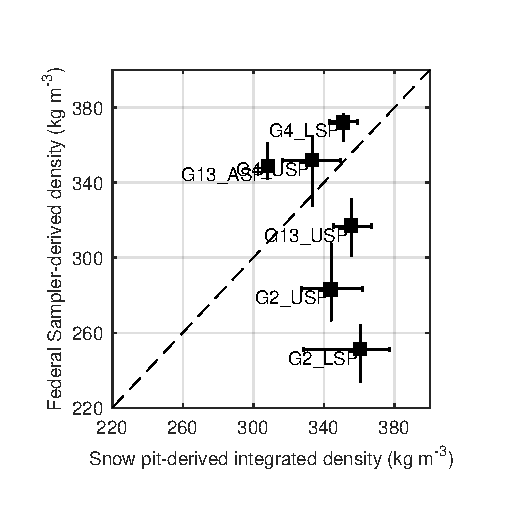
\includegraphics[width =0.5\textwidth]{SPvsFS.pdf}\\
	\caption{Comparison of integrated density estimated using wedge cutters in a snow pit and density estimated using Federal Sampler measurements for Glacier 4 (G04), Glacier 2 (G02) and Glacier 13 (G13). Snow pits were distributed in the accumulation area (ASP), upper ablation area (USP) and lower ablation area (LSP). Error bars are minimum and maximum values.}
	\label{fig:density_pitVStube}
\end{figure}

\begin{table}[]
\centering
\caption{Snow density values used for interpolating density based on snow pit (SP) densities and Federal Sampler (FS) densities. Four interpolation methods are chosen: (1) using a mean snow density for all three glaciers (Range mean density), (2) using a mean density for each glacier (Glacier mean density), (3) using a regression between density and elevation (Elevation regression), and (4) inverse-distance weighted mean density (not shown).}
\label{tab:Density}
\begin{tabular}{cccc}
 &  & \textbf{\begin{tabular}[c]{@{}c@{}}SP density\\ (kg m$^{-3}$)\end{tabular}} & \textbf{\begin{tabular}[c]{@{}c@{}}FS density\\ (kg m$^{-3}$)\end{tabular}} \\
 \midrule
\textbf{\begin{tabular}[c]{@{}c@{}}Range \\ mean density\end{tabular}} &  & 342 & 316 \\
\midrule
\multirow{3}{*}{\textbf{\begin{tabular}[c]{@{}c@{}}Glacier\\ mean density\end{tabular}}} & G4 & 348 & 327 \\
 & G2 & 333 & 326 \\
 & G13 & 349 & 307 \\
 \midrule
\multirow{3}{*}{\textbf{\begin{tabular}[c]{@{}c@{}}Elevation \\ regression\end{tabular}}} & G4 & $0.03z+274$ & $-0.16z+714$ \\
 & G2 & $-0.14z+659$ & $0.24z-282$ \\
 & G13 & $-0.20z+802$ & $0.12z+33$
\end{tabular}
\end{table}

\subsection{Grid cell average}

SWE observations within a DEM grid cell are averaged. Between one and six measurement locations are in each measured grid cell. The distribution of grid-cell SWE values for each glacier is similar to that of Figure \ref{fig:DepthBoxplot} but with fewer outliers. 

SWE measurements for each zigzag are not normally distributed about the mean SWE (Figure \ref{fig:ZigzagHistogram}). The average standard deviation of all zigzags on Glacier 4 is $\sigma_{\mathrm{G4}} =  0.027$ m w.e., on Glacier 2 is $\sigma_{\mathrm{G2}} =  0.035$ m w.e. and on Glacier 13 is $\sigma_{\mathrm{G13}} =  0.040$ m w.e.

\begin{figure}
	\centering
	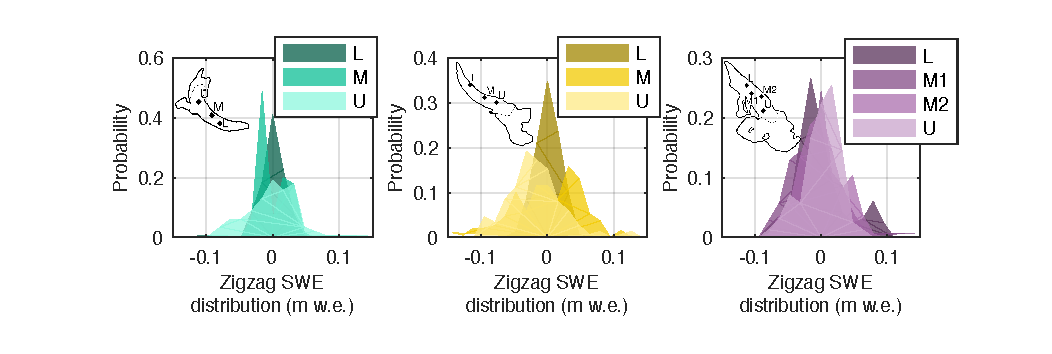
\includegraphics[width =0.5\textwidth]{ZigzagHistogram.pdf}\\
	\caption{Distribution of zigzag SWE values about the local mean on Glacier 4 (upper panel), Glacier 2 (middle panel) and Glacier 13 (lower panel). Zigzags are distributed throughout the ablation area of each glacier, with one located in the lower portion (L), one in the middle portion (M), and one in the upper portion (U). There were two zigzags in the middle ablation area of Glacier 13.}
	\label{fig:ZigzagHistogram}
\end{figure}

\subsection{Interpolated SWE}

The choice of interpolation method affects the specific WSMB (Table \ref{tab:WSMB&RMSE}). SK produces the highest WSMB on Glacier 4 and the lowest WSMB on Glacier 13. WSMB estimated by SK is $\sim$30\% lower than WSMB estimated by LR on Glaciers 2 and 13. When using LR, the WSMB on Glaciers 4 and 2 are similar in magnitude.

The predictive ability of SK and LR differ on the study glaciers. Generally, SK is better able to predict SWE at observed grid cells (Figure \ref{fig:observedVSestimated_S2}) and RMSE for all glaciers is lower for SK estimates (Table \ref{tab:WSMB&RMSE}). Glacier 13 has the lowest RMSE regardless of interpolation method, indicating lower SWE variability. The highest RMSE and the lowest correlation between estimated and observed SWE is seen on Glacier 4 (R$^2=$ 0.12) , which emphasizes the highly variable snow pack.  The highest correlation between estimated and observed SWE is on Glacier 2 when SK is used for interpolation (R$^2=$0.84) (Figure \ref{fig:observedVSestimated_S2}). Residuals for all glacier using LR and SK are normally distributed.

\begin{table}[]
\centering
\caption{Specific winter surface mass balance (WSMB [m w.e.]) estimated using linear regression and simple kriging interpolation for study glaciers. Average root mean squared error (RMSE [m w.e.]) between estimated and observed grid cells that were randomly selected and excluded from interpolation.}
\label{tab:WSMB&RMSE}
\begin{tabular}{ccccc}
 & \multicolumn{2}{c}{\textbf{Linear Regression}} & \multicolumn{2}{c}{\textbf{Simple Kriging}} \\
 & WSMB & RMSE & WSMB & RMSE \\
  \midrule
\textbf{Glacier 4} & 0.582 & 0.153 & 0.616 & 0.134 \\
 \midrule
\textbf{Glacier 2} & 0.577 & 0.102 & 0.367 & 0.073 \\
 \midrule
\textbf{Glacier 13} & 0.381 & 0.080 & 0.271 & 0.068
\end{tabular}
\end{table}

\begin{figure*}
	\centering
	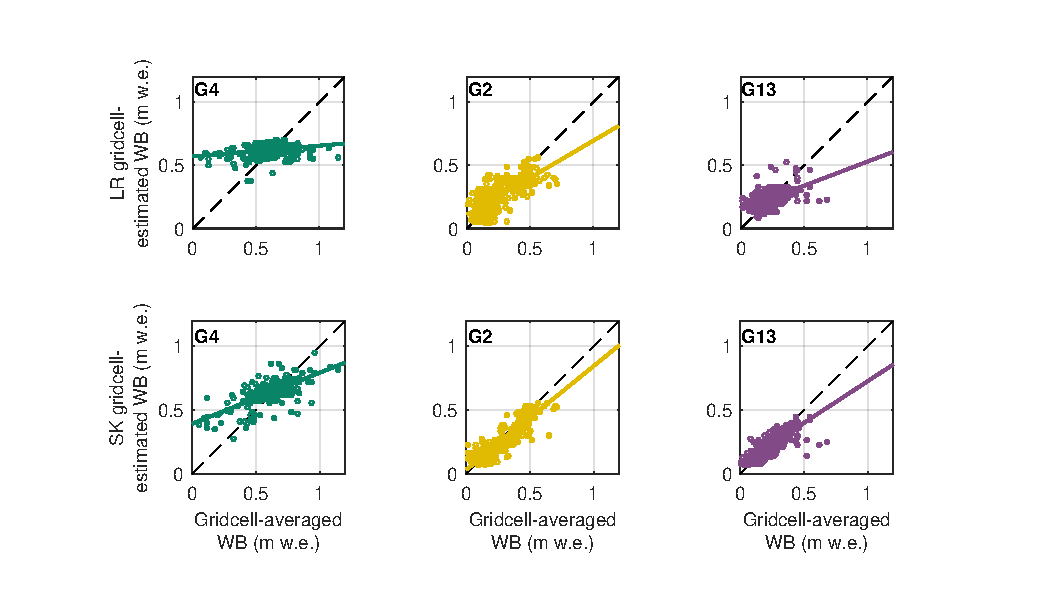
\includegraphics[width =\textwidth]{observedVSestimated_S2.pdf}\\
	\caption{Estimated grid cell SWE found using linear regression (LR) and simple kriging (SK) plotted against observed values of SWE on Glacier 4 (left), Glacier 2 (middle) and Glacier 13 (right). Line of best fit between estimated and observed SWE is also plotted.}
	\label{fig:observedVSestimated_S2}
\end{figure*}

The importance of topographic parameters in the LR differs for the three study glaciers (Figure \ref{fig:BetaCoeffs}). The most important topographic parameter for Glacier 4 is wind redistribution. However, the wind redistribution coefficient is negative, which indicates less snow in `sheltered' areas. Curvature is also a significant predictor of accumulation and the positive correlation indicates that concave down areas are more likely to have higher SWE. For Glacier 2, the most important topographic parameter is elevation, which is positively correlated with elevation. Wind redistribution is the second most important topographic parameter and has a positive correlation, which indicates that `sheltered' areas are likely to have high accumulation. The most important topographic parameter for Glacier 13 is elevation. The coefficient is positive, which means that cells at higher elevation have higher SWE. Curvature is also a significant topographic parameter but the correlation is negative, indicating less accumulation in concave areas. Most of the topographic parameters are not significant predictors of accumulation on Glacier 13. Aspect and ``northness'' are not significant predictors of accumulation on all study glaciers.

\begin{figure}
	\centering
	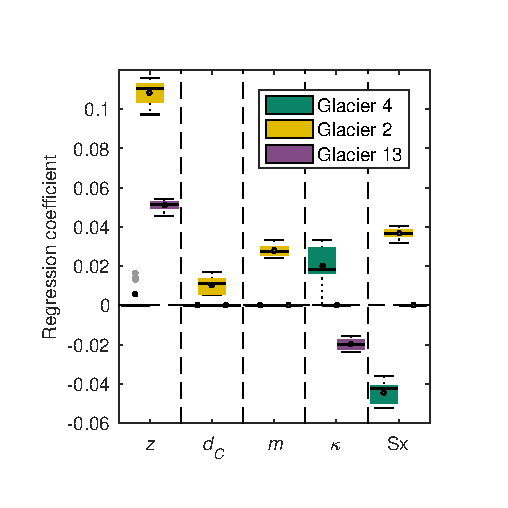
\includegraphics[width =0.5\textwidth]{BetaCoeffs.pdf}\\
	\caption{Distribution of regression coefficients for linear regression of grid cell topographic parameters and SWE calculated using eight density options on study glaciers. Topographic parameters include elevation ($z$), distance from centreline ($d_C$), slope ($m$), aspect ($\alpha$), curvature ($\kappa$), ``northness'' ($N$) and wind exposure (Sx). Regression coefficients that were not significant were assigned a value of zero.}
	\label{fig:BetaCoeffs}
\end{figure}

Spatial patterns of SWE found using LR are similar between Glaciers 2 and 13 and differ considerably for Glacier 4 (Figure \ref{fig:LR_SK_map}). Estimated SWE on Glacier 4 is relatively uniform, which results from the low predictive ability of the LR. Areas with high wind redistribution values (sheltered), especially in the accumulation area, have the lowest values of SWE. The map of modelled SWE on Glacier 2 closely matches that of elevation, which highlights the strong dependence of SWE on elevation. Glacier 2 has the largest range of estimated SWE ($0 - 1.92$ m w.e). The area of high estimated accumulation in the southwest region of the glacier  results from the combination of high elevation and Sx values. The low SWE values at the terminus are a result of low elevation and Sx values that are close to zero. The map of estimated SWE on Glacier 13 also closely follows elevation. However, the lower correlation between SWE and elevation results in a relatively small range of distributed SWE values.

There are large differences in spatial patterns of estimated WSMB for the three study glaciers found using SK (Figure \ref{fig:LR_SK_map}). On glacier, the isotropic correlation length is considerably shorter (90 m) compared to Glacier 2 (404 m) and Glacier 13 (444 m), which results in a relatively uniform SWE distribution over the glacier with small deviations at measured grid cells. Glacier 2 has two distinct and relatively uniform areas of estimated accumulation. The lower ablation area has low SWE ($\sim$0.1 m w.e.) and the upper ablation and accumulation areas have higher SWE values ($\sim$0.6 m w.e.). Glacier 13 does not appear to have any strong patterns and accumulation is generally low ($\sim0.1-0.5$ m w.e.).

SWE estimated with LR and SK differ considerably in the upper accumulation areas of Glaciers 2 and 13. The significant influence of elevation in the LR results in substantially higher SWE values at high elevation, whereas the accumulation area of the SK estimates approximate the mean observed SWE. 

\begin{figure*}
	\centering
	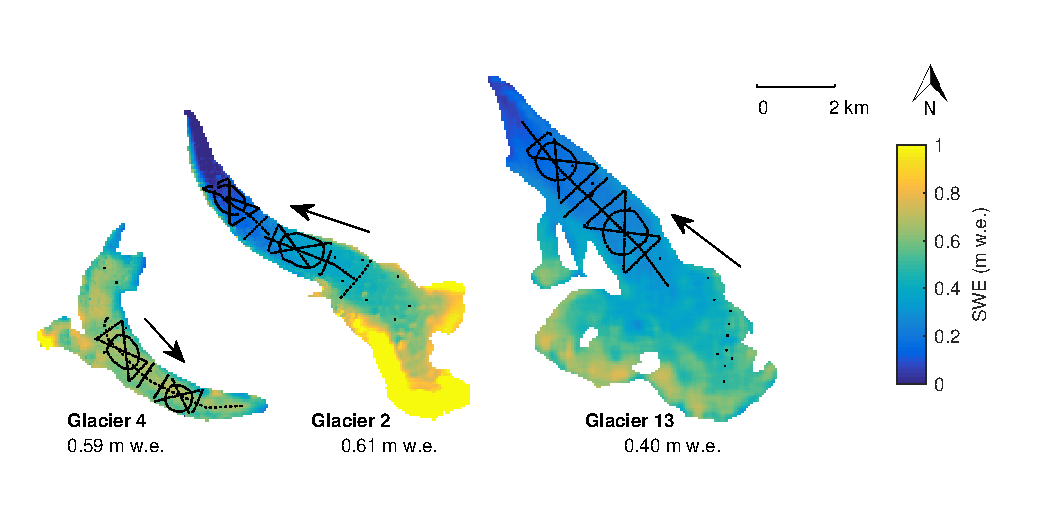
\includegraphics[width =\textwidth]{LR_map.pdf}\\
    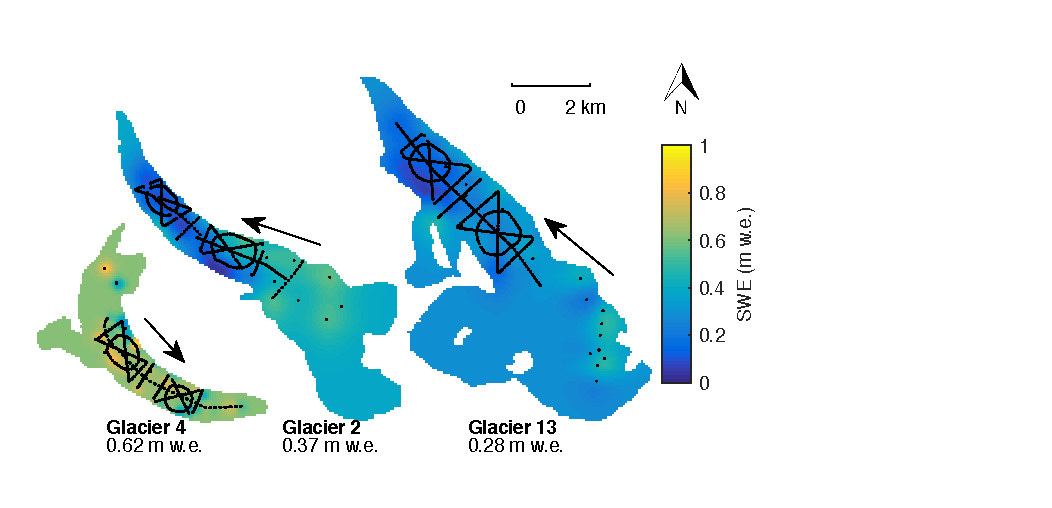
\includegraphics[width =\textwidth]{SK_map.pdf}\\
	\caption{Spatial distribution of SWE estimated using linear regression (upper) and simple kriging (lower). Grid-cell SWE observations are calculated using glacier wide mean snow pit density and are shown as black dots. Glacier flow directions are indicated by arrows. Specific WSMB values are also shown.}
	\label{fig:LR_SK_map}
\end{figure*}

Transferring LR coefficients between glaciers results in a high RMSE across the mountain range. The lowest overall RMSE (0.2051 m w.e.) results from calculating a LR using all available observations. Elevation is the only significant topographic predictor for a range-scale LR ($\beta_z=0.0525$).


\subsection{Quantifying effects of variability}

Specific WSMB is affected by variability introduced when interpolating density (density variability), when calculating grid cell SWE values (SWE variability), and when interpolating observations (interpolation variability). We find that when using a LR, $\beta$ variability has a larger effect on WSMB uncertainty than density variability or SWE variability. The probability density function (PDF) that arises from SWE variability is much narrower than the PDF that arises from interpolation variability (Figure \ref{fig:WSMBDist_LR} and Table \ref{tab:WSMBdistribution_sigma}). WSMB uncertainty found with SK interpolation is dominated by interpolation variability (Table \ref{tab:WSMBdistribution_sigma}).  

 \begin{table}[]
\centering
\caption{Standard deviation ([m w.e.]) of specific winter surface mass balance estimated using linear regression (LR) and simple kriging (SK) when variability is introduced. Density variability ($\sigma_{\rho}$) is the standard deviation of WSMB estimated using SWE data with different density interpolation methods. SWE variability ($\sigma_{\mathrm{SWE}}$) is approximated by a normal distribution about the local SWE value with standard deviation equal to the glacier-wide mean zigzag standard deviation. LR interpolation variability ($\sigma_{\beta}$) is accounted for by varying the regression coefficients with a normal distribution with standard deviation calculated from regression covariance. SK interpolation variability ($\sigma_{\mathrm{KRIG}}$) is taken from the range of distributed SWE estimates calculated by the DiceKriging package.}
\label{tab:WSMBdistribution_sigma}
\begin{tabular}{ccccccc}
\textbf{} & \multicolumn{3}{c}{\textbf{Linear Regression}} & \multicolumn{3}{c}{\textbf{Simple Kriging}} \\
 & $\sigma_{\rho}$ & $\sigma_{\mathrm{SWE}}$ & $\sigma_{\beta}$ & $\sigma_{\rho}$ & $\sigma_{\mathrm{SWE}}$ & $\sigma_{\mathrm{KRIG}}$ \\
\midrule
\textbf{G4} & 0.0190 & 0.0086 & 0.0213 & 0.0215 & 0.0085 & 0.1405 \\
\textbf{G2} & 0.0337 & 0.0180 & 0.0309 & 0.0203 & 0.0253 & 0.1378 \\
\textbf{G13} & 0.0168 & 0.0112 & 0.0280 & 0.0127 & 0.0115 & 0.0965
\end{tabular}
\end{table}

\begin{figure}
	\centering
\hspace*{-1.2cm}
	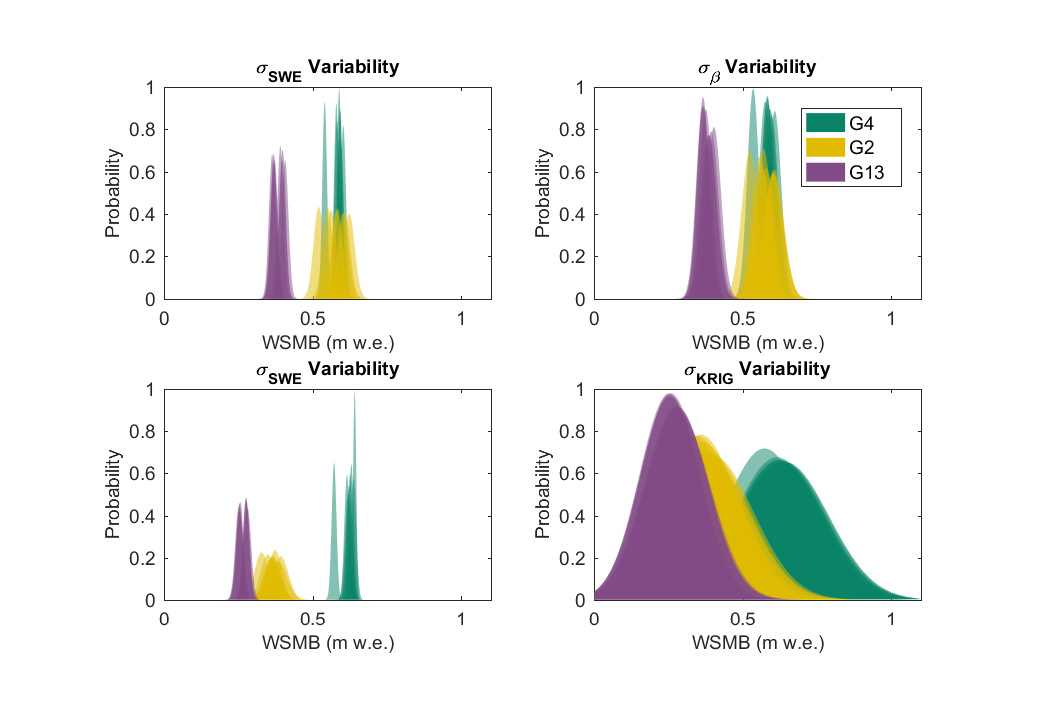
\includegraphics[width =0.62\textwidth]{WSMBDist_LR.pdf}\\
	\caption{Probability density functions (PDFs) fitted to distributions of specific winter surface mass balance (WSMB) values that arise from SWE variability ($\sigma_{ZZ}$) and regression estimation ($\sigma_{\beta}$). Each PDF is calculated using one of eight density interpolation methods for Glacier 4 (G4), Glacier 2 (G2) and Glacier 13 (G13).}
	\label{fig:WSMBDist_LR}
\end{figure}

The total WSMB uncertainty from SK interpolation is -----??---- times greater than uncertainty from LR interpolation. The PDFs overlap between the two interpolation methods although the PDF peaks are lower when SK is used for Glaciers 2 and 13 and higher for Glacier 4. SK results in WSMB distributions that overlap between glaciers and there is small probability of estimating a WSMB value of zero for Glaciers 2 and 13. LR results in overlapping WSMB distributions for Glaciers 2 and 4, with the PDF peak of Glacier 4 being slightly higher than that of Glacier 2. 

\begin{figure}
	\centering
	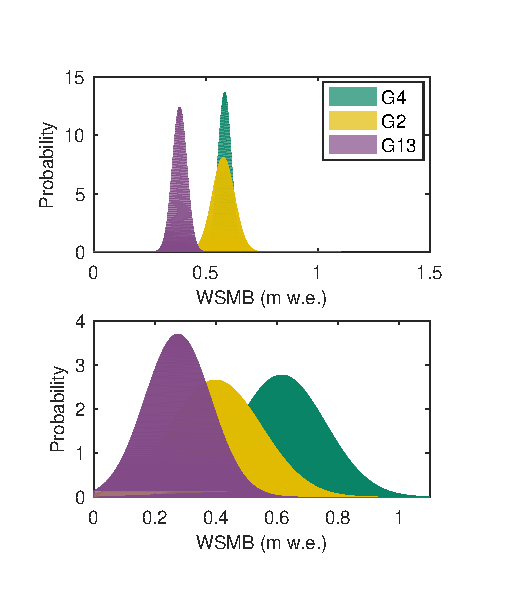
\includegraphics[width =0.5\textwidth]{WSMBDist_full.pdf}\\
	\caption{Probability density functions (PDFs) fitted to distributions of specific winter surface mass balance (WSMB) values estimated using linear regression (top) or simple kriging (bottom). Each PDF includes density variability, SWE variability and regression estimation (linear regression only) for Glacier 4 (G4), Glacier 2 (G2) and Glacier 13 (G13).}
	\label{fig:WSMBDist_LRvsSK}
\end{figure}


The spatial patterns of WSMB uncertainty are affected by density, SWE, and $\beta$ variability (Figure \ref{fig:WSMBspatialvar}).  For both LR and SK, the greatest variability in estimated SWE occurs in the accumulation area. When LR is used, estimated SWE is highly sensitive to the elevation regression parameter. In the case of SK, variability is greatest in areas far from observed SWE, which consist of the upper accumulation area on Glaciers 2 and 13. Variability is greatest on Glacier 4 when LR interpolation is used at the upper edges of the accumulation area, which correspond to the locations with extreme values of the wind redistribution parameter. When SK is used for interpolation on Glacier 4, variability is greatest at the measured grid cells, which highlights the short correlation length and the large effect of density interpolation on the SK accumulation estimate.

\begin{figure*}
	\centering
	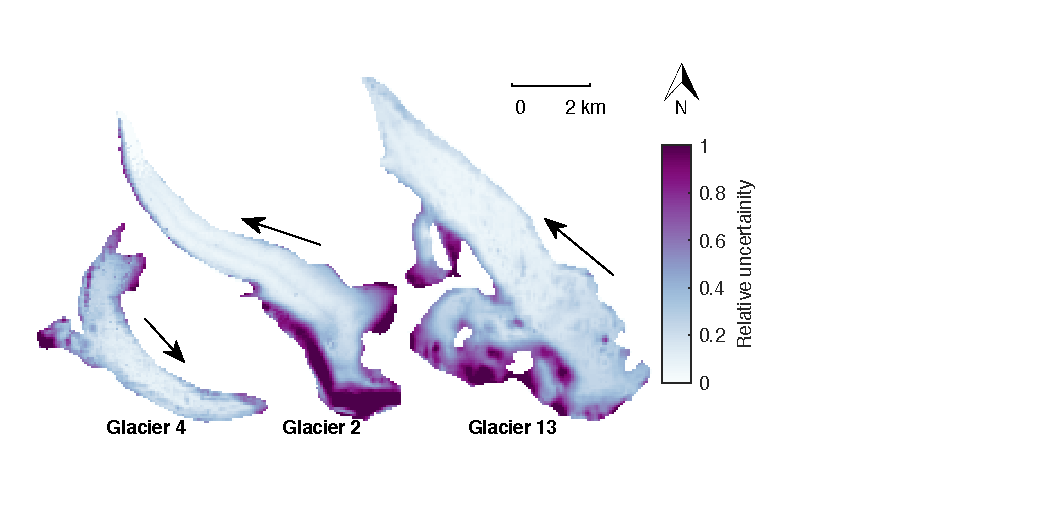
\includegraphics[width =\textwidth]{SpatialVar_LR.pdf}\\
	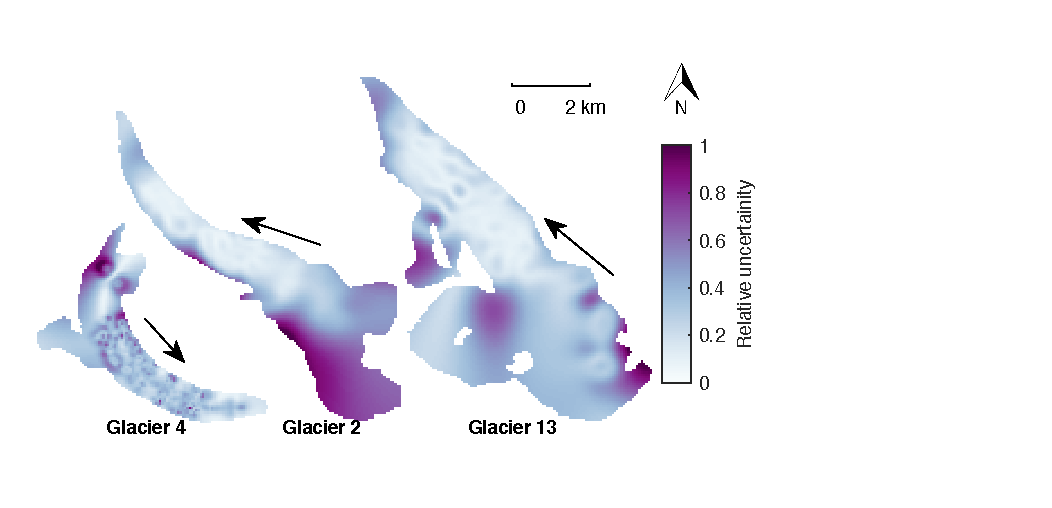
\includegraphics[width =\textwidth]{SpatialVar_SK.pdf}\\
	\caption{Variability of SWE estimated using linear regression (top) and simple kriging (bottom).	Variability is measured by taking the sum of differences between one hundred estimates of distributed WSMB that include SWE variability and, in the case of linear regression, regression variability. The sum is then normalized for each glacier.}
	\label{fig:WSMBspatialvar}
\end{figure*}



%%%%%%%%%%%%%%%%%%%%%%%%%%%%%%%%%%
% DISCUSSION
%%%%%%%%%%%%%%%%%%%%%%%%%%%%%%%%%%

\section{Discussion}

The goal of this study is to compile a comprehensive sweep of choices and assumptions present in the process of translating snow measurements to winter mass balance. The discussion focuses on evaluating the choices we made within the four main steps we needed to estimate accumulation. We then discuss the relative importance of sources of variability when estimating specific WSMB.

\subsection{Measurements}

Snow probing is the simplest and oldest method used to determine accumulation. Directl measurement of snow depth means that no data processing or corrections are needed and depth uncertainty is simple to quantify by taking multiple depth measurements close together \citep{Sold2013}. However, probing is time consuming and this limits the number of measurements that can be made. Further, measurement is limited to areas that are both accessible and safe for researchers. In complex terrain many areas cannot be surveyed, resulting in data gaps \citep{Deems2006, Sold2014}. \cite{Sold2013} noted that this systematic bias can result in incorrect values of glacier-wide accumulation, particularly because inaccessible areas such as cliffs and ridges have relatively shallow accumulations (due to wind erosion), while heavily crevassed areas can accumulate deep snow packs. Despite these limitations, we chose to use snow probing for this study to minimize cost, simplify field logistics and reduce data processing time. By focusing on simple field methods that are easy to execute, we hope to make our conclusions and recommendations for estimating WSMB more broadly applicable and reproducible.
 
Most contemporary studies that investigate glacier accumulation use ground penetrating radar (GPR), either airborne or ground-based, to obtain continuous and extensive snow depth profiles \citep[e.g.][]{Winther1998,Machguth2006, Gusmeroli2014, McGrath2015}. GPR snow surveys, especially when airborne, are able to quickly collect data over large areas and terrain accessibility does not hamper data collection. The main limitation of GPR is the misinterpretation of radargram layers, especially in areas where the snow-ice boundary is ill-defined such as the accumulation area or heavily crevassed terrain \citep{Machguth2006, Gusmeroli2014, McGrath2015}. Complications also arise when radar wave speed is altered due to varying snow density and liquid water content. Further, there is no universal procedure for obtaining snow depth data so methodology is difficult to reproduce.  Results therefore depend on available equipment, selection of processing parameters and radargram processing algorithms \citep{Sold2013}.

DEM differencing has also been used to estimate glacier-wide accumulation \citep{Deems2006,Nolan2015}. This method allows for maximal spatial data coverage. However, DEM differencing requires knowledge of glacier dynamics to account for surface changes and data collection, either by lidar or photogrammetry, is subject to considerable errors and noise \citep{Deems2006,Nolan2015}. 

Our study suffers from lack of data in the accumulation area. Snow probing cannot be used in the accumulation area because the snow-firn transition is often difficult to determine and ice lenses can be misinterpreted. Both GPR and DEM differencing are also not reliable in the accumulation area. Observe the snow-firn transition using GPR can be difficult because the density difference between snow and firn can be small. Obtaining an accurate snow surface and correlating two DEMs for differencing can also be difficult in the accumulation area because camera sensor noise and poor lighting can result in significant topographic noise. Measuring SWE in the accumulation area is difficult and subject to large errors regardless of the data collection method.

We measured snow density by sampling a snow pit (SP) and by using a Federal Sampler (FS). We found that FS and SP measurements are not correlated and that FS density values are positively correlated with snow depth. This positive relationship could be a result of physical processes, such as compaction, and/or artefacts during data collection. However, it seems more likely that this trend is a result of measurement artefacts for a number of reasons. First, the range of densities measured by the Federal sampler is large (225--410 kg m$^{-3}$) and the extreme values seem unlikely to exist at these study glaciers, which experience a continental snow pack with minimal mid-winter melt events. Second, compaction effects would likely be small at these study glaciers because of the relatively shallow snow pack (deepest measurement was 340 cm). Third, no linear relationship exists between depth and SP density (R$^2=$ 0.05). Together, these reasons lead us to conclude that the Federal Sampler measurements are biased. 

The FS appears to oversample in deep snow and undersample in shallow snow. Oversampling by small diameter (area of 10--12 cm$^2$) sampling tubes has been observed in previous studies, with a percent error between +6.8\% and 11.8\% \citep{Work1965, Fames1982, Conger2009}. Studies that use Federal Samplers often apply a 10\% correction to all measurements \citep[e.g.][]{Molotch2005}. \cite{Dixon2012} attributed oversampling to slots ``shaving'' snow into the tube as it is rotated as well as cutter deign forcing snow into the tube. \cite{Beaumont1963} found that only when snow samples had densities greater than 400 kg m$^{-3}$ and snow depth greater than 1 m, the FS oversampled due to snow falling into the greater area of slots. Undersampling is likely to occur due to snow falling out of the bottom of the sampler \citep{Turcan1975}. It is likely that this occurred during our study since a large portion of the lower elevation snow on both Glaciers 2 and 13 was melt affected and thin, allowing for easier lateral displacement of the snow as the sampler was inserted. For example, on Glacier 13 the snow surface had been affected by radiation melt (especially at lower elevations where the snow was shallower) and the surface would collapse when the sampler was inserted into the snow. It is also difficult to measure the weight of the sampler and snow with the spring scale when there was little snow because the weight was at the lower limit of what could be detected by the scale.

\subsection{Distributed density}

We choose four different density interpolation methods and keep SP and FS measurements separate. Despite the wide range of measured density values and variety in density interpolation, density does not appear to strongly affect WSMB estimates and is usually not the dominant source of WSMB uncertainty. We have relatively few density measurements throughout the study glaciers, as is common in many snow surveys, and we believe our FS measurements to be biased. Therefore, our preferred density interpolation is to use a glacier-wise mean of SP densities. This method employs common snow density measurement techniques and is easily transferable to other study areas. While using a glacier-wide mean snow density omits spatial variability in snow density \citep{Wetlaufer2016}, it does not assume unmeasured spatial correlation or trends in density.

\cite{Wetlaufer2016} found that  Distributed density from snow depth and density results in more variability than directly measuring SWE using a FS. Since SWE is more time consuming to measure than snow depth, future studies could consider decreasing the number of sample locations but directly measuring SWE to reduce the variability in  Distributed density at a measurement location. A detailed investigation of FS error is needed to contrain the variability introduces when using FS to directly measure SWE.

\subsection{Grid cell average}

\cite{Lopez2011} completed an extensive survey of snow depth variability at the plot scale (10$\times$10 m) in the Spanish Pyrenees Mountains. The authors concluded that at least five measurement points are needed in each plot to ensure estimation error is $<$10\% for plot averaged SWE. Their suggestion amounts to at least 80 measurement points for the grid cells in this study (40$\times$40 m). Rather than gridded or random sampling, as executed by the authors, we suggest a zigzag sampling scheme. The zigzag offered a comprehensive estimation of snow depth variability in a grid cell. \cite{Shea2010} proposed this linear-random sampling scheme and showed that it performs as well as pure-random sampling in detecting spatial correlations and is considerably easier to execute. 

Since such a large number of points are needed to characterize the variability in a grid cell there is little advantage to measuring and then averaging snow depth at multiple measurement locations. Rather, time should be spent extensively characterizing grid-cell variability in a few locations and to then decrease the spacing of transect measurements to extend their spatial coverage over the glacier. In our study, the grid cell variability appeared to be captured with dense sampling in select grid cells but the basin-scale variability was not captured because sampling was limited to the ablation area. By decreasing transect spacing, grid cells would only have one or two measurements but more grid cells could be measured. 

\subsection{Interpolated SWE}

Linear regression (LR) is chosen for this study because topographic parameters can be used as proxies for physical processes that affect snow distribution. Elevation was the only topographic parameter that offered relevant insight into topographic controls on accumulation. Even so, elevation had little predictive ability for Glacier 4 and the correlation was moderate on Glacier 13. Elevation affects snow distribution through melt at lower elevation due to higher temperatures, as well as increased precipitation at higher elevation arising from orographic lift. It is possible that the elevation correlation was accentuated during the field campaign due to warmer than normal temperatures and an early ($1-2$ weeks) start to the melt season (Yukon Snow Survey Bulletin and Water Supply Forecast, May 1, 2016). The southwestern Yukon winter snow pack in 2015 was also well below average, likely resulting in the effects of early melt onset to be emphasized. Glacier 4 had deeper snow and cloudier conditions during the field campaign so perhaps a correlation between SWE and elevation had not manifested. 

Our mixed insights into dominant predictors of accumulation are consistent with the conflicting results present in the literature. Many snow accumulation studies have found elevation to be the most significant predictor of SWE \citep[e.g.][]{Machguth2006, McGrath2015}. However, accumulation-elevation gradients vary considerably between glaciers \citep{Winther1998} and other factors, such as orientation relative to dominant wind direction and glacier shape, have been noted to affect accumulation distribution \citep{Machguth2006,Grabiec2011}.  \cite{Machguth2006}, \cite{Grunewald2014} and \cite{Kirchner2014} observed elevation trends in accumulation in the lower parts of their study basins but no correlation or a decrease in SWE with elevation in the upper portion of their basins. \cite{Helbig2017} suggest that an increase in accumulation with elevation can better be approximated by a power law. There are also a number of accumulation studies on glaciers that found no significant correlation between accumulation and topographic parameters and the highly variable snow distribution was attributed to complex local conditions \citep[e.g.][]{Grabiec2011,Lopez2011}.

Wind redistribution and preferential deposition of snow is known to have a large influence on accumulation at sub-basin scales. \cite{Dadic2010} used a dynamic model to show that variations in snow depth are caused by preferential deposition, which is well correlated with mean wind speed. The wind redistribution parameter used in the study was found to be a small but significant predictor of accumulation on Glacier 4 (negative correlation) and Glacier 2 (positive correlation). This result indicates that wind likely has an impact on snow distribution but that the wind redistribution parameter used in this study is perhaps not the most appropriate way to characterize the effect of wind on our study glaciers. For example, Glacier 4 is located in a curved valley with steep side walls so having a single cardinal direction for wind may be inappropriate. Examining wind redistribution parameter values that assume wind moving up or down glacier and changing direction to follow the valley could allow the wind redistribution parameter to explain more of the variance in SWE.  A universal predictor of distributed SWE therefore continues to elude researchers and accumulation variability due to interactions between glacier geometry and weather needs to be considered when estimating winter mass balance. 

Since we were unable to measure SWE in grid cells that corresponded to the extreme values of all topographic parameters, we must extrapolate linear relationships. The accumulation area, where there are few observations, is most susceptible to extrapolation errors. This area typically also has the highest SWE values, affecting the specific WSMB estimated for the glacier. In our study, the dependence of SWE on elevation, especially on Glacier 2, means that LR extrapolation results in almost 2 m w.e. estimated in the parts of the accumulation area. This exceptionally large estimate of SWE is unlikely for a continental snow pack. As described above, snow in the accumulation area has been shown to have no correlation or a negative correlation with elevation and wind effects have been observed. Therefore, extrapolating a LR that is fitted to predominantly ablation area SWE values is likely erroneous. Future studies need to focus on collecting SWE observations in the accumulation area, even if it means collecting fewer observations in the ablation area. Accumulation area observations can be used both to characterize accumulation patterns in the upper portions on a glacierized basin and to generally increase the spatial extent and topographic parameter range coverage of observations.

For all study glaciers, simple kriging (SK) is a better predictor of observed SWE. However, the WSMB uncertainty that arises from using SK is large, and unrealistic values of 0 m w.e. WSMB can be estimated. Such a large uncertainty is undesirable when estimating WSMB.  Our observations are generally limited to the ablation area so SK estimates an almost uniform distribution of SWE in the accumulation areas of the study glaciers, which is inconsistent with observations described in the literature. Extrapolation using SK is erroneous and leads to large uncertainty in estimating WSMB, which further emphasis the need for SWE observations in the accumulation area. 

SK cannot be used to understand physical processes that may be controlling snow distribution and cannot be used to estimate accumulation beyond the study area. However, a LR applied to our study glaciers resulted in little insight into dominant physical processes. Additionally, while LR can be used to predict distributed SWE in other basins, we found that transfer of LR coefficients between glaciers results in large estimation error. The LR fitted to all observed data produced the best overall predictor of SWE in the Donjek Range, so transferability of LR is also limited in our study area. Our results are consistent with \cite{Grunewald2013}, who found that local statistical models are able to perform well but  they cannot be transferred to different regions and that regional-scale models are not able to explain the majority of variance. Therefore, if the intent of a study is to estimate range-scale accumulation it is perhaps best to sparsely sample many glaciers and to make assumptions about variability within the basin rather than conducting a detailed study of one basin. The inter-basin variability in our study range is greater than the intra-basin variability (is this true???). 

A number of studies that relate SWE to topographic parameters have found success when using a regression tree interpolation model, which is a non-linear regression method \citep[e.g.][]{Elder1998, Erickson2005, Lopez2010}. Many relationships between accumulation and topographic parameters have been observed to be non-linear so regression tree are variable in snow modelling and may yield improved results \citep{Erxleben2002, Molotch2005}. 

A major assumption in our study is that RMSE is an appropriate error metric with which we can choose best models and assess their accuracy. MORE HERE!!!!


\subsection{Quantifying effects of variability}

Interpolation variability is the greatest contributor to WSMB uncertainty for both SK and LR. This uncertainty arises from extrapolation beyond the sampled region, which results in highly variability in estimated SWE in the accumulation area. To reduce WSMB uncertainty, emphasis must therefore be placed on sampling in the accumulation area and generally obtaining measurements throughout the study basin. 

SWE variability is the smallest contributor to WSMB uncertainty. Therefore, obtaining the most accurate value of SWE to represent a grid cell, even a relatively large grid cell, does not need to be a priority when designing a snow survey. Extensively measuring SWE variability in a few locations using a zigzag design appears to be a good constraint on SWE variability. However, we assume that the sampled grid cells are representative of the variability across the entire glacier, which is likely not true for areas with debris cover, crevasses and steep slopes. Effects of SWE variability in either smaller or larger grid cells could also be different so further investigation is needed.

Using a Monte Carlo experiment to propagate variability allowed us to quantify effects of variability on estimates of WSMB. However, our analysis did not include variability arising from a number of data sources. Error associated with SP and FS density measurement is not included but we believe that this error is likely to be encompassed in the wide range of density interpolation methods. DEM vertical and horizontal error are not considered in the Monte Carlo experiment mainly because there is no DEM validation data at our study location. Error associated with estimating measurement locations, which is a combination of hand-held GPS error, distance of observers from GPS and travel along a straight line, is also not considered. However, we feel that this source of error is encompassed in the variability estimated from zigzag measurements. 

While quantifying WSMB uncertainty is an important feature of accumulation studies, we also need to consider how much uncertainty we are willing to accept. At what point do we say that we are not able to make an accurate estimate of WSMB? In our study, are we able to say that our most probable estimate of WSMB found using SK is appropriate to report when the uncertainty is so large? Further, is our assumption that we have captured the majority of uncertainty in our variability analysis sufficient? 

\subsection{Mountain range accumulation gradient}

An accumulation gradient is observed for the continental side of the St. Elias Mountains (Figure \ref{fig:AccumGrad}). Accumulation data is compiled from \cite{Taylor1969}, the three glaciers presented in this paper, as well as two snow pits we dug at the head of the Kaskawalsh Glacier in May 2016. The data show a linear decrease in observed SWE with distance from the main mountain divide identified by \citep{Taylor1969} with a gradient of $-0.024$ m w.e. km$^{-1}$. This relationship indicates that glacier location within a mountain range also affects glacier-wide WSMB. Interaction between meso-scale weather patterns and mountain topography is a major driver of glacier-wide accumulation. Further insight into mountain-scale accumulation trends can be achieved by investigating moisture source trajectories and orographic precipitation contribution to accumulation. 


\begin{figure}
	\centering
	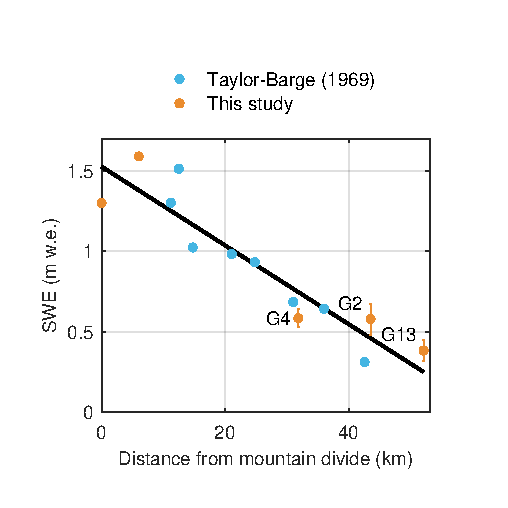
\includegraphics[width =0.5\textwidth]{AccumGrad.pdf}\\
	\caption{Relation between SWE and linear distance from St. Elias mountain divide, located at the head of the Kaskawalsh Glacier. Blue dots are snow pit derived SWE values from \citep{Taylor1969}. Orange dots farthest from the divide are mean WSMB from Glaciers 4, 2 and 13, with 95\% confidence interval using a linear regression interpolation. Orange dots close to the divide are snow pit derived SWE value at two locations in the accumulation area of the Kaskawalsh Glacier collect in May 2016. Black line indicates line of best fit (R$^2=0.85$).}
	\label{fig:AccumGrad}
\end{figure}


\subsection{Limitations and future work}

Extensions to this work could include an investigation of experimental design, examining implications of a non-linear SWE elevation trend, examining the effects of DEM grid size on WSMB and resolving temporal variability. 

Our sampling design was chosen to extensively sample the ablation area and is likely too finely resolved for many future mass balance surveys to replicate. Therefore, it is valuable to investigate how best to reduce our sampling design and measurement spacing while maintaining a reasonable estimate of distributed WSMB. \cite{Lopez2010} examined data reduction in a $\sim$6 km$^2$ basin and found a non-linear response of model stability and accuracy to sample size. The authors concluded that $200-400$ observations are needed to obtain accurate and robust models. Determining a sampling design that minimizes error and reduces the number of measurements, known as data efficiency thresholds, would contribute to optimizing snow surveys in mountainous regions. 

A non-linear SWE-elevation trend has been documented in a number of studies so it would be valuable to further investigate this relationship. Although more observations in the accumulation area are needed to confirm this relationship on our study glaciers, we could apply a variety of non-linear elevation trends to investigate their effects on WSMB estimates. 

DEM grid cell size had a large influence on the resolution of topographic features \citep{Lopez2010} , which can have implications for calculating a LR. DEM grid cell size is known to significantly affect computed topographic parameters and the ability for a DEM to resolve important hydrological features (i.e. drainage pathways) in the landscape \citep{Zhang1994, Garbrecht1994, Guo-an2001}. \cite{Zhang1994} found that simulating geomorphic and hydrological process for many landscapes is best accomplished with a 10-m grid cell size, which is an optimal compromise between increasing resolution and large data volumes. The authors found that a 30- and 90-m grid cell size were insufficient in resolving terrain features in a  moderately to steep gradient topography. \cite{Lopez2010} state that a grid cell size of 5 m is need for a reliable representation of terrain and to accurately identity solar radiation, curvature and slope. The authors conclude that relevant topographic parameters in their $\sim$6 km$^2$ basin are completely lost at grid sizes greater than $55\times55$ m making DEMs with a coarse resolution inappropriate for modelling snow packs. Further, the importance of topographic parameters in predicting SWE was correlated with DEM grid size. A decrease in spatial resolution of the DEM resulted in a decrease in the importance of curvature and an increase in the importance of elevation and, to a lesser degree, solar radiation. These results corroborated \cite{Kienzle2004}, who found that curvature was the main predictor of SWE with a high resolution DEM. To further confound the use of DEMs to estimate SWE, \cite{Molotch2005} found that estimated SWE distributions were dependent on the DEM chosen. Even different DEMs with similar spatial resolutions can generate significantly different topographic parameters and resulting SWE distributions. A detailed DEM is therefore needed to identify the features that drive accumulation variability. 

Future studies could also evaluate the effects of DEM uncertainty on elevation and derived topographic parameters. \cite{Wechsler2006} used a Monte Carlo experiment to quantify deviation of topographic parameters due to DEM error. The authors found that elevation did not significantly deviate but slope and other hydrological parameters such as catchment area and topographic index were significantly affected. \cite{Guo-an2001} also conducted an DEM error analysis and found that the accuracy of hydrological topographic parameters was closely related to the the vertical resolution of the DEM. Errors were especially large in smooth plain areas with slope less than 4 degrees.

It appears then that topographic parameters included in a LR and the uncertainty in estimating WSMB are dependant on the resolution of DEM grid cells. Future accumulation investigations should therefore focus on obtaining a high resolution DEM and quantifying effects of DEM variability on WSMB. There is a strong need for a better understanding of the effects of DEM error and grid size on glacier accumulation. The majority of published studies focus on hydrological modelling and the study areas are non-glacierized. Glacier present different accumulation patterns and surface topography so the DEM resolution and uncertainty may also differ.

Temporal variability in accumulation is not considered in our study. While this limits the extent of our conclusions, a number of studies have found temporal stability in spatial patterns of snow accumulation and that terrain-based model could be applied reliable between years \citep[e.g.][]{Grunewald2013}. For example, \cite{Walmsley2015} analyzed more than 40 years of accumulation record on two Norwegian glaciers and found that snow accumulation is spatially heterogeneous yet exhibits robust time stability in distributions. Reliability maps were then used to reduce the sampling scheme to one index site as well as a transect with 50 m elevation intervals for each glacier and winter balance was estimated to with 0.15 m w.e. However, the temporal transferability of terrain-based parameterization is not always reliable. \cite{Walmsley2015} also found several strongly irregular snow spatial distribution years that were inconsistent with the overall reduced sampling schemes.\cite{Revuelto2014} also noted that snow distribution variability could not be explained by their model in low snow years.

%%%%%%%%%%%%%%%%
\section{Introduction}

Objective: (1) Discuss choices made when moving from measurement to accumulation and (2) show how system variability and our choices interact to create uncertainty in our estimate of accumulation

- snow distribution in alpine regions is not uniform or static, but
rather highly variable and influenced by diverse and dynamic processes operating on multiple spatial and temporal scales -> topographic effects (crevasses, surface topo, elevation aspect, precip grad across range), snow drift and preferential deposition
-  [22] note that studies of snow water equivalent (SWE) that have been conducted in
alpine environments vary considerably in the extent and spacing of their measurements.
- Snow accumulation is spatially variable on point scales (<5 m), hillslope scales (1–100 m),
basin scales (100–10,000 m) and regional scales (10–1000 km) [22].
-Point-scale variability is generally associated with surface roughness effects and the
presence of small obstacles. -> take three measures
Many parts of a glacier though
are characterized by a relatively smooth surface, with roughness lengths on the order of
centimeters [57]. In these areas, point-scale variability of snow depth is low. However, in
heavily crevassed regions, point-scale variability can be large and thus exert a dominant
control on snow distribution in the area [82].
-Hillslope-scale variability is caused by variations in the surface topography of the glacier.
The curvature and slope of the surface as well as the presence of local ridges or depressions
can affect where snow is located [15, 115]. Avalanching can also redistribute snow, especially
on the margins of a glacier [17, 89].
Watershed-scale variability results mainly from the effects of changing elevation and
aspect on atmopsheric conditions [22]. In particular, orographic lifting and shading can
result in higher elevation and north-facing areas of the glacier having more snow than other
areas [89, 115]. Gradients in temperature from elevation changes also affect the freezing
level, which determines whether precipitation falls as snow or rain [17]. For example, [77]
found a strong influence of elevation in determining accumulation on Findel Glacier in
Switzerland.
Regional variability occurs when areas within a mountain range have differing amounts of
snow. Often, this results from horizontal precipitation gradients and rain shadows forming
on the lee side of topographic divides. Areas with large, steep mountains are especially
affected by these processes.

----------------------------------------------------

derived accumulation
estimated winter surface mass balance
distributed snow water equivalent
%------------------------------------------------



%----------------------------------------------------------------------------------------
%	REFERENCE LIST
%----------------------------------------------------------------------------------------
%
\bibliography{/home/glaciology1/Documents/MastersDocuments/MastersLit}
\bibliographystyle{igs}

%----------------------------------------------------------------------------------------

\end{document}
